\section{The turning solution, its duration and the averaged null energy}\label{rep:turning}

With a constant vacuum energy $3\MPbar^2h^2$ the negative Casimir energy turns a contracting torus around along an exact, regular, time-symmetric solution.
We derive it (Sec.~\ref{rA:turn-solution}), compute the conformal duration of the turn in closed form (Sec.~\ref{rA:turn-duration}), show that the solution is null geodesically complete and find its averaged null energy in closed form (Secs.~\ref{rA:turn-complete}--\ref{rA:turn-anec}), and calibrate it with the plateau inflaton of assumption~\ref{assump:A3} (Sec.~\ref{rA:turn-plateau}).
For the Standard Model with its zero-mode energy the torus turns around at an edge of $\Lb=722\,\MPbar^{-1}$, about $3.6\times10^3$ Planck lengths, and each branch lasts $\eta_\infty=1.31103/(\rAHeff\Lb)\simeq300$ light-crossing times in conformal time. %

\subsection{The leading solution}
\label{rA:turn-solution}

At leading order the shape is the cube, the inflaton sits on its plateau, and the energy density is the sum of a vacuum energy and the Casimir energy with its zero-mode part,
\begin{equation}
\rho=3\MPbar^2h^2-\frac{C_{\rm eff}}{L^4},\qquad C_{\rm eff}=\rANeff\rAgam=(1-\fzm)\NC\rAgam .
\label{eq:rA-rho-turn}
\end{equation}
The Friedmann constraint of Eq.~\eqref{eq:rA-einstein} with $S=0$, $3\MPbar^2H^2=\rho$, becomes an equation for $y\equiv L^2$:
\begin{equation}
\dot y^2=4H^2y^2=4h^2y^2-\frac{4C_{\rm eff}}{3\MPbar^2}=4h^2\big(y^2-\Lb^4\big),\qquad \Lb^4=\frac{C_{\rm eff}}{3\MPbar^2h^2}.
\end{equation}
Its regular solution with $\dot y=0$ at $t=0$ is $y=\Lb^2\cosh2ht$, that is~\cite{Zeldovich:1984vk,Guth:2025dal}
\begin{equation}
L=\Lb\sqrt{\cosh2ht},\qquad \Lb^4=\frac{\rANeff\rAgam}{3\MPbar^2h^2},
\label{eq:rA-turning-solution}
\end{equation}
with
\begin{equation}
H=h\tanh2ht,\qquad \dot H=2h^2\,{\rm sech}^22ht .
\label{eq:rA-H-turn}
\end{equation}
The second Einstein equation is satisfied as well: the Casimir stress is traceless, so $\rho+\bar p=\tfrac43\rho_C=-\tfrac43C_{\rm eff}/L^4$ and $\dot H=\tfrac23C_{\rm eff}/(\MPbar^2L^4)=2h^2\Lb^4/L^4$, which is Eq.~\eqref{eq:rA-H-turn}.
The universe contracts for $t<0$, turns at $t=0$ with $\dot H=2h^2>0$, and expands for $t>0$; at $|t|\gg1/h$ it approaches de~Sitter space with $L\simeq\Lb e^{h|t|}/\sqrt2$.
The leading solution was found by Zel'dovich and Starobinsky~\cite{Zeldovich:1984vk} and written in closed form by Guth and Vilenkin~\cite{Guth:2025dal}.
McInnes~\cite{McInnes:2005sa} used the same solution for a pre-inflationary torus and discarded its contracting half as a redundant dual description.
Mithani and Vilenkin~\cite{Mithani:2014toa} found turning points of a flat Casimir torus in which matter with $w=-2/3$ takes the place of the vacuum energy.
Here both halves are physical (assumption~\ref{assump:A4}), and Fig.~\ref{fig:rA-turning} shows them with the arrows of time of the two-branch reading of Sec.~\ref{rep:gate}.

\begin{figure}[tbp]
\centering
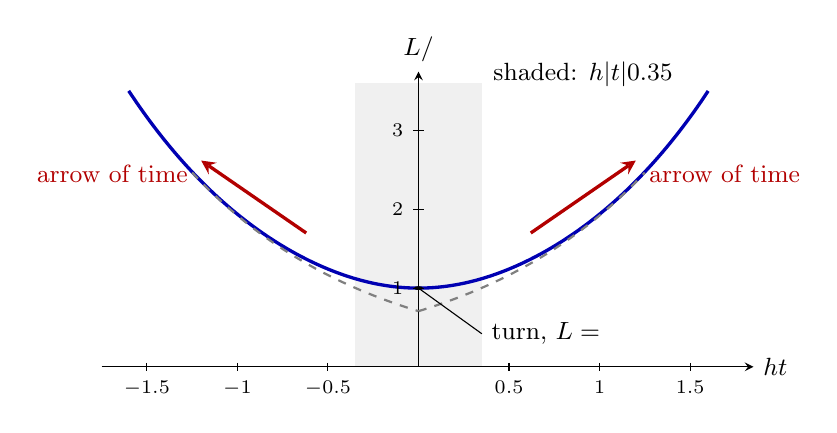
\begin{tikzpicture}[xscale=2.3,yscale=1.0,>=stealth]
  \fill[gray!12] (-0.35,0) rectangle (0.35,3.6);
  \draw[->] (-1.75,0) -- (1.85,0) node[right] {\small $ht$};
  \draw[->] (0,0) -- (0,3.75) node[above] {\small $L/\Lb$};
  \draw[very thick,blue!70!black,domain=-1.6:1.6,samples=81,smooth] plot (\x,{sqrt(cosh(2*\x))});
  \draw[dashed,gray,thick,domain=0:1.25,samples=40] plot (\x,{exp(\x)/sqrt(2)});
  \draw[dashed,gray,thick,domain=-1.25:0,samples=40] plot (\x,{exp(-\x)/sqrt(2)});
  \draw[very thick,->,red!70!black] (0.62,1.70) -- (1.20,2.62);
  \draw[very thick,->,red!70!black] (-0.62,1.70) -- (-1.20,2.62);
  \node[red!70!black,right] at (1.22,2.45) {\small arrow of time};
  \node[red!70!black,left] at (-1.22,2.45) {\small arrow of time};
  \fill (0,1) circle (0.025);
  \draw[thin] (0,1) -- (0.35,0.42);
  \node[right] at (0.35,0.42) {\small turn, $L=\Lb$};
  \node[right] at (0.36,3.72) {\small shaded: $h|t|\lesssim0.35$};
  \foreach \xx in {-1.5,-1,-0.5,0.5,1,1.5} \draw (\xx,0.05) -- (\xx,-0.05) node[below] {\scriptsize $\xx$};
  \foreach \yy in {1,2,3} \draw (0.03,\yy) -- (-0.03,\yy) node[left] {\scriptsize $\yy$};
\end{tikzpicture}
\caption{The turning solution, Eq.~\eqref{eq:rA-turning-solution}, and its two-branch reading.
The edge $L$ of the cubic torus contracts, turns at $L=\Lb$ and re-expands; dashed: the de~Sitter asymptotes $\Lb e^{h|t|}/\sqrt2$.
In the two-branch reading (assumption~\ref{assump:A4}, Sec.~\ref{rep:gate}) both halves are futures of the turning point, with arrows of time pointing away from it.
The shaded band marks the window $h|t|\lesssim0.35$ within which a real Gaussian shape state must be set for the shape to survive on both branches with probability $90\%$ (Sec.~\ref{rep:quantum-shape}).}
\label{fig:rA-turning}
\end{figure}

\subsection{Conformal time and the duration of the turn}
\label{rA:turn-duration}

The Higgs zero mode and the light fields evolve in conformal time $\eta$, $dt=L\,d\eta$, in which a light ray crosses the torus once per unit of $\eta$.
Along Eq.~\eqref{eq:rA-turning-solution}
\begin{equation}
\eta(t)=\int_0^t\frac{dt'}{L(t')}=\frac{1}{h\Lb}\int_0^{ht}\frac{d\tau}{\sqrt{\cosh2\tau}} ,
\end{equation}
which converges as $t\to\pm\infty$ because the integrand falls as $\sqrt2\,e^{-|\tau|}$.
Each branch therefore lasts a finite conformal time,
\begin{equation}
\eta_\infty=\frac{1}{h\Lb}\int_0^\infty\frac{d\tau}{(\cosh2\tau)^{1/2}}=\frac{1}{2h\Lb}\int_0^\infty{\rm sech}^{1/2}x\,dx=\frac{\Gamma(\tfrac14)^2}{4\sqrt{2\pi}\,h\Lb}=\frac{1.31103}{h\Lb},
\label{eq:rA-etainf}
\end{equation} %
where we used $\int_0^\infty{\rm sech}^\nu x\,dx=\tfrac12\sqrt\pi\,\Gamma(\tfrac\nu2)/\Gamma(\tfrac{\nu+1}2)$ at $\nu=\tfrac12$ and $\Gamma(\tfrac14)\Gamma(\tfrac34)=\sqrt2\,\pi$.
The number $1.31103$ is half the lemniscate constant, for a reason that the conformal-time form of the solution makes plain.

\paragraph{Lemniscatic form.}
In conformal time, with $a\equiv L$ and $a'=da/d\eta=La\,H$, the constraint reads $a'^2=a^4H^2=h^2(a^4-\Lb^4)$.
For $Y\equiv a^2$ this becomes $Y'^2=4h^2Y(Y^2-\Lb^4)$, a cubic in $Y$.
With $Y=\Lb^2\,\wp(z)$ and $z=h\Lb\,\eta$ it takes the Weierstrass form $\wp'^2=4\wp^3-g_2\wp-g_3$ with $g_2=4$ and $g_3=0$, the lemniscatic case:
\begin{equation}
L(\eta)^2=\Lb^2\,\wp\big(h\Lb(\eta-\eta_0);4,0\big),
\label{eq:rA-lemniscatic}
\end{equation}
with the turn at the real half period, where $\wp=e_1=1$.
The scale factor diverges at the two poles of $\wp$ that bound the real period, so the whole history spans the finite conformal interval $2\omega_1/h\Lb$, with $\omega_1=\int_1^\infty dt/\sqrt{4t^3-4t}=1.31103$, in agreement with Eq.~\eqref{eq:rA-etainf}. %
The same variables give the identity
\begin{equation}
\frac{a''}{a}=\dot a^2+a\ddot a=a^2\big(2H^2+\dot H\big)=2h^2a^2
\label{eq:rA-app}
\end{equation}
along the whole solution, by Eq.~\eqref{eq:rA-H-turn}: the turning point acts on minimally coupled fields exactly as de~Sitter space does, because the Casimir stress is traceless.
Sections~\ref{rep:gate} and~\ref{rep:spectra} use Eq.~\eqref{eq:rA-app}; with Eq.~\eqref{eq:rA-lemniscatic} it turns the mode equation of a minimally coupled field into the Lam\'e equation $d^2v/dz^2=[2\wp(z)-k^2/(h\Lb)^2]v$.

\paragraph{The duration used in the Higgs chapters.}
On the plateau the rate of the cosh solution is $\rAHeff$ rather than $h$ (Sec.~\ref{rA:turn-plateau}), so the conformal duration of one branch is $\eta_\infty=1.31103/(\rAHeff\Lb)$.
The Higgs calculation uses $\rAHeff\Lb=0.00437243$, which gives $\eta_\infty=299.84$ in units of $1/L$. %
This is the duration of the turn that enters the survival of the Higgs zero mode (Sec.~\ref{rep:h-survival}); the threshold depends on it only logarithmically (Sec.~\ref{rep:h-universality}).
The constant $\rAHeff\Lb$ of the Higgs calculation and the plateau ratio $h\Lb=0.0044$ of the benchmark differ by the factor $0.98949$ and must not be interchanged. %
Most of a branch is spent near the turn: half of $\eta_\infty$ elapses by $ht=0.76$, $64\%$ by the onset of shape freezing at $ht\simeq1.09$, and $90\%$ by $ht=2.38$, after which the integrand falls as $\sqrt2\,e^{-ht}$. %

\subsection{Null completeness and the violation of the null energy condition}
\label{rA:turn-complete}

The solution is null geodesically complete.
Along a null geodesic with conserved comoving momentum $\bm p$, the physical frequency is $\omega=|\bm p|/L$ and the affine parameter obeys $d\lambda=L\,dt/|\bm p|$.
Since $\int L\,dt=\Lb\int\sqrt{\cosh2ht}\,dt$ diverges at both ends, every null geodesic has infinite affine length in both directions.
By Corollary~3.3 of Ref.~\cite{Zhou:2026szo}, a non-static Bianchi~I spacetime that obeys the null energy condition has every null geodesic incomplete, so the Casimir state must violate that condition.
It does: $\rho+p=\tfrac43\rho_C<0$.

\subsection{The averaged null energy}
\label{rA:turn-anec}

The averaged null energy along every null geodesic quantifies the violation, and we find it in closed form.
For the isotropic leading background $R_{kk}\equiv R_{\mu\nu}k^\mu k^\nu=(\rho+p)\,\omega^2/\MPbar^2$ with $\rho+p=\tfrac43\rho_C=-\tfrac43C_{\rm eff}/L^4$, and Eq.~\eqref{eq:rA-turning-solution} gives $C_{\rm eff}/(\MPbar^2\Lb^4)=3h^2$.
With $d\lambda=dt/\omega$ and $\omega=|\bm p|/L$,
\begin{equation}
\begin{aligned}
\int R_{kk}\,d\lambda&=\frac{1}{\MPbar^2}\int(\rho+p)\,\omega\,dt=-\frac{4C_{\rm eff}|\bm p|}{3\MPbar^2}\int\frac{dt}{L^5}=-4h^2|\bm p|\Lb^4\int\frac{dt}{L^5}\\
&=-\frac{4h^2|\bm p|}{\Lb}\int_{-\infty}^{\infty}\frac{dt}{(\cosh2ht)^{5/2}}=-2h\,\omega_b\int_{-\infty}^{\infty}{\rm sech}^{5/2}x\,dx,
\end{aligned}
\label{eq:rA-anec-integral}
\end{equation}
with $\omega_b=|\bm p|/\Lb$ the null frequency at the turning point.
Since $\int{\rm sech}^{5/2}x\,dx=\sqrt\pi\,\Gamma(\tfrac54)/\Gamma(\tfrac74)$ and $\Gamma(\tfrac54)/\Gamma(\tfrac74)=\tfrac{\frac14\Gamma(\frac14)}{\frac34\Gamma(\frac34)}=\Gamma(\tfrac14)^2/(3\sqrt2\,\pi)$,
\begin{equation}
\int R_{kk}\,d\lambda=-\frac{\sqrt2\,\Gamma(1/4)^2}{3\sqrt\pi}\,h\,\omega_b=-3.4961\,h\,\omega_b . %
\label{eq:rA-anec}
\end{equation}
The result is negative for every null geodesic and proportional to its frequency at the turn.

\paragraph{The averaged sum rule.}
The violation satisfies the averaged sum rule $I_p=-J_p$ that Proposition~4.1 of Ref.~\cite{Zhou:2026szo} establishes for complete null geodesics, where $I_p=\int R_{kk}\,d\lambda$ and $J_p=\int\Tr B_p^2\,d\lambda$.
The optical tensor is $B_p=\omega H\,\rAone_2$, so $J_p=2|\bm p|\int H^2L^{-1}dt$.
On the solution this is
\begin{equation}
J_p=\frac{2|\bm p|h^2}{\Lb}\int\frac{\tanh^22ht}{(\cosh2ht)^{1/2}}\,dt=h\,\omega_b\int\big({\rm sech}^{1/2}x-{\rm sech}^{5/2}x\big)dx=2h\,\omega_b\int{\rm sech}^{5/2}x\,dx,
\end{equation}
because $\int{\rm sech}^{1/2}x\,dx=\sqrt\pi\,\Gamma(\tfrac14)/\Gamma(\tfrac34)$ is exactly three times $\int{\rm sech}^{5/2}x\,dx$.
Hence $I_p=-J_p$ holds analytically on the leading solution; numerical quadrature confirms it to $2\times10^{-16}$. %
The identity is the integrated null Raychaudhuri equation, $d(\Tr B_p)/d\lambda=-\Tr B_p^2-R_{kk}$, whose boundary term $\Tr B_p=2\omega H$ vanishes at both ends because $\omega\to0$.

\paragraph{Achronal averaged null energy condition.}
Every null geodesic of the torus winds around it and is not achronal, so this violation is consistent with the achronal averaged null energy condition, the version free of known violations by quantum fields~\cite{Graham:2007va}.

\subsection{The plateau turning point and its calibration}
\label{rA:turn-plateau}

For the plateau of Eq.~\eqref{eq:rA-plateau} the turning point sits at an inflaton value $\phi_b$ with $H=\dot\phi=0$, and the history is time symmetric.
At the turn the vacuum energy is $V(\phi_b)$, which replaces $h$ in Eq.~\eqref{eq:rA-turning-solution} by
\begin{equation}
\rAHeff=\frac{1}{\MPbar}\Big[\frac{V(\phi_b)}{3}\Big]^{1/2}=\big(1-e^{-\sqrt{2/3}\,\phi_b/\MPbar}\big)\,h=0.9895\,h ;
\label{eq:rA-Heff}
\end{equation} %
the numbers below include this factor.
Elsewhere we measure time in units of $1/h$, $\tau\equiv ht$, because the $1\%$ difference is below the accuracy of every result that uses Eq.~\eqref{eq:rA-turning-solution}, except the shape thresholds of Sec.~\ref{rep:quantum-shape}, which are in units of $1/\rAHeff$.

\paragraph{Calibration.}
We fix $h$ by the observed scalar amplitude and the pivot $k_*=0.05\,{\rm Mpc}^{-1}$ by thermal matching. %
With instant reheating this gives $N_*=55.722$ e-folds between pivot exit and the end of inflation and $h/\MPbar=6.116\times10^{-6}$ (Sec.~\ref{rep:spectra}). %
For the AAA Standard Model with free fields and a reference present torus side $L_0=6/H_0$, $0.96$ times the diameter $\dLSS$ of the last-scattering sphere, a pivot solver gives $\phi_b=5.5794\,\MPbar$, $N_{\rm post}=68.25$ e-folds after the turning point and $h\Lb=0.00483$. %
The solver integrates the background from the turn with the inflaton released at $\phi_b$, finds the end of inflation and the e-fold at which $k_*$ leaves the Hubble radius, and adjusts $\phi_b$ so that the comoving torus scale today is $L_0$.
The present size enters only through $\ln L_0$: for $0.95\leq L_0/\dLSS\leq2$ the turning-point quantities $V(\phi_b)$ and $h\Lb$ change by at most $2.2\times10^{-4}$, while $N_{\rm post}$ grows by $\ln(L_0H_0/6)$. %

\paragraph{The benchmark.}
With free fields Eq.~\eqref{eq:rA-turning-solution} gives $(\Lb\MPbar)^4=\NC\rAgam/[3(\rAHeff/\MPbar)^2]$, that is $\Lb\MPbar=790$. %
The zero-mode energy replaces $\NC$ by $\rANeff$ in Eq.~\eqref{eq:rA-turning-solution}, which lowers $\Lb$ by the factor $(1-\fzm)^{1/4}=0.9147$, or $8.5\%$. %
The benchmark turning point therefore has
\begin{equation}
\Lb\MPbar=722,\qquad h\Lb=0.0044, %
\label{eq:rA-benchmark}
\end{equation}
and the matching scale of assumption~\ref{assump:A2} is $\mub=1/\Lb=\MPbar/722=3.37\times10^{15}$\,GeV. %
At fixed $L_0$ the factor $0.9147$ acts like a change of $\ln L_0$ by $0.09$, so $V(\phi_b)$ changes by less than $10^{-4}$ and $N_{\rm post}$ grows by $0.09$. %
Table~\ref{tab:rA-fzero} collects the background quantities with and without the zero-mode energy.

\begin{table}[tbp]
\centering
\caption{Background quantities for free fields ($\fzm=0$) and with the leading-order zero-mode energy ($\fzm=0.30$, the benchmark). %
$\rANeff=(1-\fzm)\NC$; $\Lb$ and $h\Lb$ refer to the plateau history of this chapter; $\kappa_E$ and $\kappa_{T_2}$ are the normalized stiffnesses of the aspect and angle modes at the cube (Sec.~\ref{rep:shape}).
The first next-order corrections lower $\fzm$ to $0.28$ and $\kappa_E$ to $18.0$ ($\kappa_{T_2}=-8.34$).} %
\label{tab:rA-fzero}
\begin{tabular}{lcc}
\toprule
 & $\fzm=0$ & $\fzm=0.30$\\ %
\midrule
$\rANeff$ & $25.5$ & $17.9$\\ %
$\Lb\MPbar$ & $790$ & $722$\\ %
$h\Lb$ & $0.0048$ & $0.0044$\\ %
$\kappa_E$; $\kappa_{T_2}$ & $13.53$; $-6.35$ & $19.32$; $-9.07$\\ %
\bottomrule
\end{tabular}
\end{table}

\subsection{Scales of the turning point}
\label{rA:turn-scales}

The benchmark torus is $\Lb=722\sqrt{8\pi}\,\ell_{\rm P}\simeq3.6\times10^3$ Planck lengths, or $6\times10^{-32}$\,m, across, about $230$ times smaller than the Hubble radius $1/h$. %
The small parameter of the semiclassical description is
\begin{equation}
\epsilon=\sqrt{\NC}\,\frac{h}{\MPbar}=\sqrt{\frac{3}{\rAgam}}\,(h\Lb)^2\simeq3\times10^{-5},
\label{eq:rA-epsilon}
\end{equation} %
where the second form, with the free-field $\Lb$ and the rate of the cosh solution in place of $h$, follows from $(\rAHeff\Lb)^4=\NC\rAgam\rAHeff^2/3\MPbar^2$; the two forms differ by the $1\%$ between $h$ and $\rAHeff$.
It is the squared ratio of the light-crossing time of the torus to the Hubble time at the turn, up to the factor $\sqrt{3/\rAgam}=1.338$, the factor with which the finite-volume shape inertia of Sec.~\ref{rep:shape} enters.
Anomalous corrections to the criterion~\eqref{eq:rA-exact-criterion} are of relative order $\epsilon^2$.
The turning point is also slow compared with the photon gap: the lowest photon pair has the frequency $4\pi/\Lb$, and the adiabaticity parameter of the turn is $(h\Lb/4\pi)^2\simeq1.2\times10^{-7}$, so the lowest photon modes follow it adiabatically (Sec.~\ref{rep:gate}). %
All modes of the torus are inside the Hubble radius at the turn by at least the factor $2\pi/(h\Lb)\simeq1400$ (1300 for free fields; Sec.~\ref{rep:spectra}). %
